\chapter{Landasan Teori}
\label{chap:landasanteori}

Bab ini terdiri atas empat bagian, yaitu Google Authentication, Markdown Syntax, StrapdownJS dan Zurb Foundation. Empat bagian terebut akan membahas mengenai dasar-dasar teori mengenai Google Authentication, Markdown Syntax, StrapdownJS dan Zurb Foundation yang akan digunakan dalam penelitian ini untuk membangun perangkat lunak Sistem Informasi Riwayat Mahasiswa.

\section{Google Authentication \cite{Oauth:2013}}
\label{sec:googleauthentication}

API Google menggunakan protokol OAuth 2.0 untuk otentikasi dan otorisasi. OAuth 2.0 adalah protokol yang relatif sederhana. Untuk memulainya cukup dengan mendapatkan kepercayaan OAuth 2.0 dari Google Developers Console\footnotemark[1]. Maka aplikasi akan meminta suatu token akses dari Google Authorization Server, ekstrak token akses yang merupakan jawaban dari server, dan mengirim token akses ke Google API yang akan diakses.

\footnotetext[1]{https://console.developers.google.com/}
\footnotetext[2]{https://developers.google.com/accounts/docs/OpenIDConnect}

Sub bab berikut memberikan gambaran skenario otorisasi OAuth 2.0 yang merupakan dukung dari Google. Rincian tentang cara menggunakan OAuth 2.0 untuk otentikasi (yaitu sign-in), dapat dilihat pada OpenID Connect\footnotemark[2].

\subsection{Langkah Dasar}
Semua aplikasi akan mengikuti pola dasar ketika menggakses Google API menggunakan Oauth 2.0. Terdapat empat langkah yang harus diikuti :

\begin{enumerate}
\item
Mendapatkan kepercayaan OAuth 2.0 dari Google Developers Console\\
Berkunjung ke Google Developers Console untuk mendapatkan kepercayaan OAuth 2.0 seperti klien id dan kerahasiaan klien yang keduanya dikenal oleh Google dan aplikasi yang dibuat. Set nilai-nilai yang bervariasi sesuai dengan jenis aplikasi apa yang sedang dibuat. Misalnya, sebuah aplikasi javascript tidak memerlukan sebuah rahasia, tapi apakah aplikasi web server memerlukannya.
\item
Memperoleh token akses dari Google Authorization Server\\
Sebelum aplikasi dapat mengakses data privat dengan menggunakan Google API, terlebih dahulu diperlukan token akses untuk mengakses API tersebut. Satu token akses dapat memberikan berbagai tingkat akses ke beberapa API. Izin token akses merupakan parameter untuk variabel ruang lingkup yang mengontrol sumber daya dan operasi. Selama ada permintaan untuk token akses, maka aplikasi akan mengirimkan satu atau lebih nilai pada parameter ruang lingkup.

Ada beberapa cara dan variasi untuk melakukan permintaan tersebut berdasarkan aplikasi yang dibangun. Contohnya aplikasi JavaScript mungkin meminta token akses menggunakan mesin pencari yang mengarah kembali ke Google, namun aplikasi yang dibangun diinstal pada perangkat tidak memiliki fitur mesin pencari maka akan menggunakan {\it web service}. Beberapa permintaan memerlukan tahap otentikasi dimana pengguna diharuskan login menggunakan akun Google mereka. Setelah login pengguna akan ditanya apakah pengguna akan memberi izin untuk aplikasi yang telah melakukan permintaan tersebut. Proses ini disebut izin dari pihak pengguna. Jika pengguna memberi izin, maka Google Authorization Server akan mengirimkan aplikasi tersebut sebuah token akses. Jika pengguna tidak memberi izin, maka server akan menunjukan respon yang menyatakan eror.
\item
Kirim token akses ke API\\
Setelah aplikasi mendapat token akses, lalu aplikasi akan mengirimkan token akses ke Google API melalui otorisasi yang terletak pada header HTTP. Sangat mungkin untuk mengirimkan token sebagai parameter permintaan URI dalam tipe data {\it string}, namun langkah ini tidak direkomendasikan karena parameter URI akan berakhir pada file log yang tidak aman. Juga merupakan hal yang baik karena menghindari menciptakan nama parameter URI yang tidak perlu.
Token akses hanya berlaku untuk set operasi dan sumber daya yang dijelaskan pada lingkup permintaan token. Sebagai contoh, jika token akses dikeluarkan untuk Google+ API, hal tersebut tidak memberikan akses untuk Google Contact API. Namun token akses untuk Google+ API dapat dikirim beberapa kali untuk operasi yang serupa.
\item
Memperbaharui token akses jika diperlukan\\
Token akses memiliki daya tahan yang terbatas. Jika aplikasi yang dibangun membutuhkan akses ke Google API melebihi masa aktif token akses, maka dapat memperbaharui token akses tersebut. Hal ini memungkinkan untuk memdapatkan token akses yang baru.
\end{enumerate}

\subsection{Skenario Google Authentication}
Terdapat lima skenario yang dapat digunakan untuk Google Authentication yaitu Skenario Aplikasi Web Server, Skenario Aplikasi yang Terinstal, Skenario Aplikasi Sisi Klien (JavaScript), Skenario Aplikasi Pada Perangkat Dengan Masukan Yang Terbatas, dan Skenario Layanan Akun. Untuk penjelasan lebih lanjut dapat dilihat pada sub-sub-bab berikut.

\subsubsection{Skenario Aplikasi Web Server}
Google OAuth 2.0 mendukung aplikasi web server yang menggunakan bahasa dan kerangka kerja seperti PHP, Java, Python, Ruby, dan ASP.NET.

Urutan otorisasi dimulai ketika aplikasi mengarahkan mesin pencari ke URL Google; URL tersebut termasuk parameter permintaan yang menunjukkan jenis akses yang diminta. Google menangani otentikasi pengguna, pemilihan sesi, dan izin dari pihak pengguna. Hasilnya adalah sebuah kode otorisasi, dimana aplikasi dapat bertukar untuk token akses dan memperbaharui token akses.

Aplikasi harus menyimpan pembaharuan token akses untuk penggunaan kedepannya dan menggunakan token akses untuk mengakses Google API. Setelah masa token akses berakhir, maka aplikasi akan memperbaharui token akses untuk mendapatkan yang baru. Untuk gambaran skenario dapat dilihat pada Gambar \ref{fig:skenarioaplikasiwebserver}.

\begin{figure}[H]
\centering
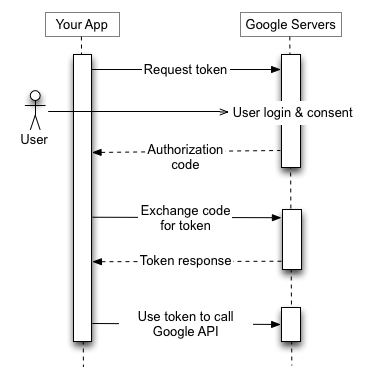
\includegraphics[scale=1]{Gambar/skenario1.png}
\caption[Gambar Skenario Aplikasi Web Server]{Skenario Aplikasi Web Server} 
\label{fig:skenarioaplikasiwebserver}
\end{figure}

\subsubsection{Skenario Aplikasi yang Terinstal}
Google OAuth 2.0 mendukung aplikasi yang diinstal pada perangkat seperti komputer, perangkat mobile, dan tablet. Ketika membuat klien id melalui Google Developers Console, menentukan aplikasi yang terinstal kemudian pilih Android, Chrome, iOS, atau "{\it Other}" sebagai jenis aplikasi.

Hasil proses klien id dan kerahasiaan klien dalam beberapa kasus dimasukkan dalam kode sumber aplikasi. (Dalam konteks ini, kerahasiaan klien jelas tidak diperlakukan sebagai rahasia.)

Urutan otorisasi dimulai ketika aplikasi mengarahkan mesin pencari ke URL Google; URL termasuk parameter permintaan yang menunjukkan jenis akses yang diminta. Google menangani otentikasi pengguna, pemilihan sesi, dan izin pengguna. Hasilnya adalah sebuah kode otorisasi yang dapat bertukar untuk token akses dan memperbaharui token.

Aplikasi harus menyimpan token yang diperbaharui untuk penggunaan masa depan dan menggunakan token akses untuk mengakses API Google. Setelah masa token akses berakhir, maka aplikasi akan memperbaharui token untuk mendapatkan yang baru. Untuk gambar skenario dapat dilihat pada Gambar \ref{fig:skenarioaplikasiyangterinstal}.

\begin{figure}[H]
\centering
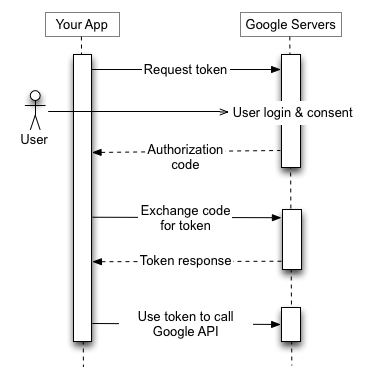
\includegraphics[scale=1]{Gambar/skenario1.png}
\caption[Gambar Skenario Aplikasi yang Terinstal]{Skenario Aplikasi yang Terinstal} 
\label{fig:skenarioaplikasiyangterinstal}
\end{figure}

\subsubsection{Skenario Aplikasi Sisi Klien (JavaScript)}
Google OAuth 2.0 mendukung aplikasi JavaScript yang berjalan di mesin pencari. Urutan otorisasi dimulai ketika aplikasi mengarahkan mesin pencari ke URL Google; URL termasuk parameter permintaan yang menunjukkan jenis akses yang diminta. Google menangani otentikasi pengguna, pemilihan sesi, dan izin pengguna. Hasilnya adalah token akses dimana klien harus memvalidasi sebelum memasukkannya ke dalam permintaan Google API. Ketika masa token berakhir, aplikasi mengulangi proses. Untuk gambar skenario dapat dilihat pada Gambar \ref{fig:skenarioaplikasisisiklien}.

\begin{figure}[H]
\centering
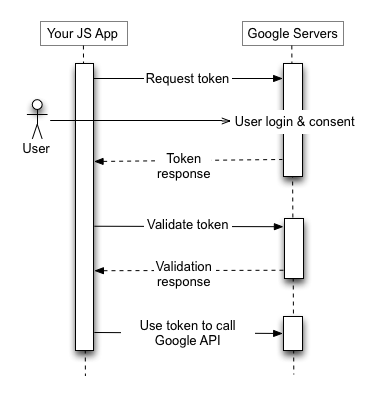
\includegraphics[scale=1]{Gambar/skenario2.png}
\caption[Gambar Skenario Aplikasi Sisi Klien (JavaScript)]{Skenario Aplikasi Sisi Klien (JavaScript)}
\label{fig:skenarioaplikasisisiklien}
\end{figure}

\subsubsection{Skenario Aplikasi Pada Perangkat Dengan Masukan Yang Terbatas}
Google OAuth 2.0 mendukung aplikasi yang berjalan pada perangkat dengan masukan yang terbatas seperti konsol game, kamera video, dan printer. Urutan otorisasi dimulai dengan aplikasi membuat permintaan layanan web ke URL Google untuk kode otorisasi. Tanggapan berisi beberapa parameter, termasuk URL dan kode bahwa aplikasi menunjukkan kepada pengguna. Pengguna memperoleh URL dan kode dari perangkat, kemudian beralih ke perangkat terpisah atau komputer dengan kemampuan masukan yang lebih. Pengguna membuka mesin pencari, menavigasi ke URL tertentu, melakukan log in, dan memasukan kode.

Sementara itu, aplikasi jajak pendapat dari URL Google pada interval tertentu. Setelah pengguna menyetujui akses, respon dari server Google berisi token akses dan memperbaharui token. Aplikasi harus menyimpan token yang baru untuk penggunaan masa depan dan menggunakan token akses untuk mengakses Google API. Setelah masa token akses berakhir, maka aplikasi akan memperbaharui token untuk mendapatkan yang baru. Untuk gambar skenario dapat dilihat pada Gambar \ref{fig:skenarioaplikasimasukanterbatas}.

\begin{figure}[H]
\centering
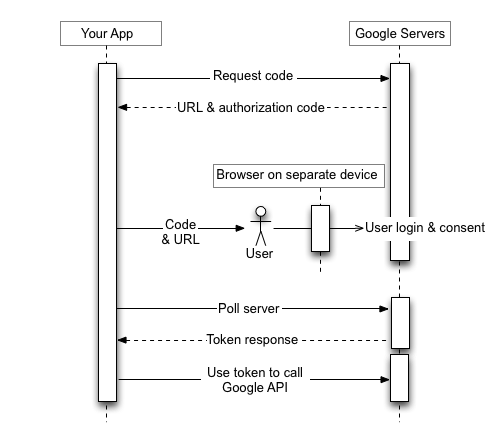
\includegraphics[scale=1]{Gambar/skenario3.png}
\caption[Gambar Skenario Aplikasi Pada Perangkat Dengan Masukan Yang Terbatas]{Skenario Aplikasi Pada Perangkat Dengan Masukan Yang Terbatas}
\label{fig:skenarioaplikasimasukanterbatas}
\end{figure}

\subsubsection{Skenario Layanan Akun}
Google API seperti Prediction API dan Google Cloud Storage dapat bertindak atas nama aplikasi yang dibuat tanpa mengakses informasi pengguna. Dalam situasi ini aplikasi perlu membuktikan identitasnya sendiri ke API, tapi tidak diperlukan izin dari pihak pengguna. Demikian pula, dalam skenario perusahaan, aplikasi dapat meminta akses didelegasikan ke beberapa sumber daya.

Untuk jenis interaksi antara server memerlukan layanan akun, dimana akun tersebut terdapat pada aplikasi yang dibuat, bukan individu ke pengguna akhir. Aplikasi memanggil Google API atas nama layanan akun, dan izin dari pihak pengguna tidak diperlukan. (Dalam skenario tanpa layanan akun, aplikasi memanggil Google API atas nama pengguna akhir, dan izin dari pihak pengguna kadang-kadang diperlukan.)

Catatan: skenario layanan akun ini membutuhkan aplikasi untuk membuat dan tanda kriptografi JSON Web Token (JWTs). Sangat disarankan untuk menggunakan perpustakaan untuk melakukan tugas-tugas ini. Jika menulis kode ini tanpa menggunakan perpustakaan secara abstrak tanda penciptaan dan penandatanganan, mungkin membuat kesalahan yang akan memiliki dampak yang parah pada keamanan aplikasi yang dibangun.

Kredensial ayanan akun , yang diperoleh dari Google Developers Console, termasuk alamat email yang dihasilkan yang unik, klien id, dan setidaknya satu pasang kunci publik / privat. Menggunakan klien id dan satu kunci privat untuk membuat JWT ditandatangani dan membangun permintaan token akses dalam format yang sesuai. Aplikasi kemudian mengirimkan permintaan token ke Google OAuth 2.0 Authorization Server, yang mengembalikan token akses. Aplikasi menggunakan token untuk mengakses API Google. Ketika masa token berakhir, aplikasi mengulangi proses. Untuk gambar skenario dapat dilihat pada Gambar \ref{fig:skenariolayananakun}.

\begin{figure}[H]
\centering
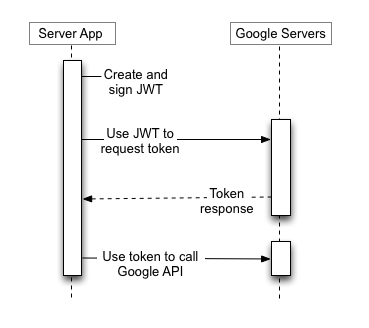
\includegraphics[scale=1]{Gambar/skenario4.png}
\caption[Gambar Skenario Layanan Akun]{Skenario Layanan Akun}
\label{fig:skenariolayananakun}
\end{figure}

\subsection{Masa Habis Berlaku Token}
Kode token harus ditulis untuk mengantisipasi kemungkinan bahwa token yang diberikan mungkin tidak lagi bekerja suatu saat. Token mungkin berhenti bekerja untuk beberapa alasan di bawah ini:

\begin{itemize}
\item
Pengguna telah mencabut akses.
\item
Token tidak digunakan selama enam bulan.
\item
Akun pengguna telah melampaui jumlah tertentu permintaan token.
\end{itemize}

Saat ini batas untuk setiap akun Google adalah 25 token. Jika pengguna akun telah memiliki 25 token, permintaan otentikasi untuk token ke-26 akan berhasil tapi token yang paling tua atau token ke-1 akan dibuat tidak berlaku tanpa sepengetahuan pengguna.
Jika perlu untuk mengotorisasi beberapa program, mesin, atau perangkat, salah satu solusi adalah untuk membatasi jumlah klien dimana harus mengotorisasi per pengguna akun antara 15 atau 20. Jika Anda adalah admin Google Apps, Anda dapat membuat admin tambahan untuk mengizinkan beberapa klien.

\subsection{Lingkup Otorisasi}
Lingkup disini merupakan sebuah string yang memungkinkan akses ke sumber daya tertentu, misalnya akses ke data pengguna. Dengan memasukan lingkup tertentu pada saat permintaan otorisasi, kemudian mendapatkan izin sesuai dengan teks yang akan ditampilkan ke pengguna. Setelah mendapat persetujuan dari pihak pengguna untuk izin atas lingkup tersebut, maka Google mengirimkan token untuk aplikasi yang mengidentifikasi untuk memberikan otorisasi khusus. Dengan kata lain, lingkup dan token menentukan apa saja data pengguna yang diberi izin oleh pengguna untuk diakses.

Sebuah aplikasi yang dibuat tanpa permintaan otentikasi (tidak ada lingkup yang diminta) hanya dapat mengakses data pengguna yang umum di Google+. Contoh, jika sebuah aplikasi mencari postingan publik, respon dari pencarian akan menampilkan id pengguna yang telah diposting secara publik dan aplikasi dapat mengakses nama dan URL foto pengguna yang dimana keduanya selalu diposting secara publik. Dapat juga mengakses tanggal ulang tahun atau jenis kelamin pengguna jika pengguna telah mempostinng secara publik. Untuk daftar lingkup otorisasi dapat dilihat pada sub-sub-bab berikut.

\subsubsection{Lingkup Profil}
Lingkup ini merupakan lingkup dasar dimana lingkup ini melakukan beberapa hal seperti berikut:
\begin{itemize}
\item
Meminta agar aplikasi diberikan akses ke informasi profil dasar bagi pengguna yang terotentikasi.
\item
Memungkinkan aplikasi untuk mengetahui siapa pengguna yang dikonfimasi dengan mengganti id pengguna dengan "me" yang mewakilkan pengguna yang telah terotentikasi disetiap permintaan yang dilakukan.
\item
Memungkinkan aplikasi diakses melalui aplikasi android.
\end{itemize}
\begin{lstlisting}
https://www.googleapis.com/auth/plus.login
\end{lstlisting}
Lingkup login disarankan menyediakan akses ke fitur sosial. Lingkup ini secara implisit mencakup lingkup profil dan juga meminta aplikasi diberikan akses ke:
\begin{itemize}
\item
Rentang usia pengguna yang telah terotentikasi.
\item
Daftar teman yang telah diberikan akses oleh pengguna.
\item
Metode untuk membaca, menulis dan menghapus kegiatan app ke Google atas nama pengguna.
\end{itemize}
Memungkinkan lintas platform dengan pendaftaran tunggal.

\subsubsection{Lingkup Email}
Lingkup ini meminta agar aplikasi diberikan akses ke:
\begin{itemize}
\item
Alamat email akun Google dari pengguna. Mengakses alamat email dengan memanggil people.get yang akan mengeluarkan array email atau dengan memanggil people.getOpenIdConnect yang akan mengeluarkan email dengan format OIDC.
\item
Nama domain Google Apps jika ada yang dimiliki pengguna. Nama domain dikembalikan sebagai kepemilikan domain dari people.get atau properti hd dari getOpenIdConnect.
\end{itemize}
Lingkup email ini setara dengan lingkup yang lain:
https://www.googleapis.com/auth/plus.me.

\subsubsection{Lingkup yang lain}
Lingkup openid menginformasikan server otorisasi bahwa klien membuat permintaan OpenID Connect dan meminta akses ke id pengguna yang terotentikasi tersebut. Lingkup ini harus disertakan lingkup OpenId Connect.

Metode getOpenIdConnect mengembalikan profil pengguna dengan format OIDC mengikuti jalur permintaan HTTP:
https://www.googleapis.com/plus/v1/people/me/openIdConnect.

\begin{lstlisting}
https://www.googleapis.com/plus/v1/people/me/openIdConnect
\end{lstlisting}
Untuk keperluan login menggunakan profil atau lingkup
\begin{lstlisting}
https://www.googleapis.com/auth/plus.login
\end{lstlisting}
karena lingkup
\begin{lstlisting}
https://www.googleapis.com/auth/plus.me
\end{lstlisting}
tidak dianjurkan sebagai lingkup login dikarenakan pengguna yang belum upgrade ke Google+ tidak akan mengembalikan nama atau alamat email pengguna.

Lingkup ini melakukan hal berikut:
\begin{itemize}
\item
Memungkinkan aplikasi untuk mengetahui siapa pengguna yang dikonfimasi dengan mengganti id pengguna dengan "me" yang mewakilkan pengguna yang telah terotentikasi disetiap permintaan yang dilakukan.
\end{itemize}

\subsubsection{Lingkup yang tidak dipakai lagi}
\begin{lstlisting}
https://www.googleapis.com/auth/userinfo.profile
\end{lstlisting}
Ganti dengan lingkup yang setara yaitu lingkup profil. Lingkup ini setara dengan lingkup profil dan meminta akses data yang sama.

Catatan: lingkup ini tidak dipakai lagi namun tetap dipertahankan dan terus tersedia untuk kompatibilitas.

\begin{lstlisting}
https://www.googleapis.com/auth/userinfo.email
\end{lstlisting}
Ganti dengan lingkup yang setara yaitu lingkup email. Lingkup ini meminta akses ke alamat email akun Google pengguna.
Google menghasilkan token baru dengan lingkup ini untuk titik akhir people.get. Lingkup ini juga meminta akses dari pengguna ke titik akhir userinfo unutk kompatibilitas.

Lihat juga lingkup terkait:
\begin{lstlisting}
https://www.googleapis.com/auth/plus.profile.emails.read
\end{lstlisting}

Catatan: lingkup ini tidak dipakai lagi namun tetap dipertahankan dan terus tersedia untuk kompatibilitas.

\section{Markdown}
\label{sec:markdown}

\subsection{Apa itu Markdown? \cite{Markguide:2015}}
John Gruber pembuat Markdown, memperkenalkan Markdown sebagai alat konfersi sebuah teks untuk ditampilkan ke HTML untuk para penulis website. Markdown memungkinkan penulis mudah untuk membaca dan mudah untuk menulis sebuah teks biasa, lalu merubah teks tersebut secara struktural yang valid dengan XHTML atau HTML.
Markdown memiliki beberapa sintaks yang sederhana sebagai peraturan dalam menulis, hal tersebut membuat mudah dalam konfersi ke HTML dengan banyak perangkat lunak yang mendukung.
Untuk contoh, jika menulis **hello** pada Markdown dan konfersi ke HTML menggunakan teks editor yang mendukung, teks tersebut akan menjadi <strong>hello</hello> yang akan terlihat \textbf{hello}.

\subsection{Sintaks yang Berguna \cite{Markguide:2015}}
Terdapat beberapa sintaks untuk penggunaan cetak tebal, cetak miring, judul sub bab, batas garis, paragraf, gambar, link, kode, kutipan, garis horisontal, dan list. Untuk penjelasan lebih lanjut dapat dilihat pada sub sub bab di bawah ini.

\subsubsection{Cetak Tebal dan Cetak Miring}
Markdown memperlakukan karakter bintang (*) sebagai penekanan. Teks yang dibungkus dengan satu karakter * maka hasil teks akan cetak miring, dan teks yang dibungkus dengan dua karakter * maka hasil teks akan cetak tebal.
\begin{lstlisting}
*hello* untuk cetak miring
**hello** untuk cetak tebal
\end{lstlisting}

\subsubsection{Judul Bab}
Markdown memperlakukan karakter hash (\#) sebagai indikator dari bab. Gunakan beberapa karakter hash untuk bab. Selalu gunakan spasi antara karakter hash dengan teks yang akan digunakan. Jumlah \# yang digunakan akan menentukan ukuran judul bab.
\begin{lstlisting}
# Judul Bab (an <h1> tag)
## Judul Sub Bab (an <h2> tag)
### Judul Sub Sub Bab (an <h3> tag)
#### Tingkat ke 4 (an <h4> tag)
##### Tingkat ke 5 (an <h5> tag)
###### Tingkat ke 6 (an <h6> tag)
\end{lstlisting}

\subsubsection{Batas Baris}
Untuk menyisipkan satu baris baru dalam dokumen, mengakhiri baris dengan dua atau lebih spasi lalu tekan 'Enter'.
\begin{lstlisting}
Baris ini dengan   
batas baris
\end{lstlisting}
Contoh di atas, setelah kata 'dengan' diakhiri dengan tiga spasi lalu tekan 'Enter'.
\begin{lstlisting}
Baris ini tanpa
batas baris
\end{lstlisting}
Contoh di atas, setelah kata 'tanpa' diakhiri tanpa spasi langsung tekan 'Enter'.

\subsubsection{Paragraf}
Untuk menyisipkan paragraf baru, cukup menyisipkan satu baris kosong.
\begin{lstlisting}
Ini kalimat pertama. Ini kalimat berikutnya. Ini kalimat terakhir.

Ini paragraf baru.
\end{lstlisting}
Contoh diatas baris pertama adalah peragraf kesatu. Setelah itu ada satu baris kosong. Kalimat kedua merupakan paragraf kedua.

\subsubsection{Gambar}
Untuk menyisipkan gambar pada dokumen Markdown, gunakan sintaks berikut
\begin{lstlisting}
![teks](/url_gambar "judul_gambar")
\end{lstlisting}
Contoh penggunaan sintaks gambar: 
\begin{lstlisting}
![logo](https://www.google.com/images/srpr/logollw.png "Google")
\end{lstlisting}
Url gambar dapat diganti dengan path yang mengarah pada file gambar yang akan digunakan.

\subsubsection{Link}
Untuk menyisipkan hyperlink pada dokumen Markdown, gunakan sintaks berikut 
\begin{lstlisting}
[link_teks](/tujuan_url "judul opsional")
\end{lstlisting}
Contoh penggunaan sintaks link:
\begin{lstlisting}
[my_website](http://browsernative.com "Click Here")
\end{lstlisting}

\subsubsection{Kode}
Untuk menyisipkan kode pada sebuah baris pada dokumen Markdown, gunakan karakter kutip belakang ('). Lampirkan kode yang ingin disisipkan dalam karakter kutip belakang. Untuk menyisipkan blok kode gunakan tiga kutip belakang ('''). Setiap baris kode harus diawali dengan empat spasi.
\begin{lstlisting}
Definisi dari 'initLabels()' dapat dilihat di bawah ini"

'''
    function initLabels(){
        function setLabels(elementId, messageId){
            var label = document.querySelector('label[for=' + elementId + ']');
            label.textContent = chrome.i18n.getMessage(messageId);
        }
    }
'''

Paragraf lain.
\end{lstlisting}
'initLabels()' akan menjadi kode pada satu baris kalimat. Sedangkan fungsi yang ada didalam ''' akan menjadi blok kode.

\subsubsection{Kutipan}
Untuk menyisipkan kutipan pada dokumen Markdown, gunakan tanda lebih besar (>) pada awal kupitan.
\begin{lstlisting}
Ini merupakan kutipan **favorit** saya:

> The weak can never forgive.
> Forgiveness is the attribute of the strong.
\end{lstlisting}

\subsubsection{Garis Horisontal}
Menyisipkan garis horisontal pada dokumen Markdown, gunakan tiga atau lebih tanda hubung (-) dalam baris baru. Maka akan muncul sebagai garis horisontal pada keluaran HTML.
\begin{lstlisting}
# Bagian Satu

The quick brown fox jumps over the lazy dog. The quick brpwn fox jump over the lazy dog.

---

Last Edited on *25th Dec 2014*
\end{lstlisting}
Pada contoh di atas --- akan menjadi garis horisontal.

\subsubsection{Daftar}
Terdapat dua macam daftar yang dapat dibuat. Dua macam daftar tersebut dapat dilihat dibawah ini.

\begin{enumerate}
\item Daftar tidak berurutan\\
Untuk membuat daftar tidak berurutan dapat menggunakan simbol bintang *, simbol tambah +, maupun tanda hubung - sebelum daftar item yang ingin dimasukkan. Untuk contoh penggunaan dapat dilihat di bawah ini.
\begin{lstlisting}
* Item
* Item
* Item

+ Item
+ Item
+ Item

- Item
- Item
- Item
\end{lstlisting}
\item Daftar berurutan\\
Untuk membuat daftar berurutan dapat menggunakan nomor sebelum daftar item yang ingin dimasukkan. Untuk contoh penggunaan dapat dilihat di bawah ini.
\begin{lstlisting}
1. Item 1
2. Item 2
3. Item 3
\end{lstlisting}

\subsection{GitHub Flavored Markdown \cite{Markdown:2015}}
GitHub menggunakan "GitHub Flavored Markdown" atau disingkat menjadi GFM. GFM berbeda dengan Standar Markdwon (SM) dalam beberapa bagian yang cukup signifikan dan ada beberapa sintaks tambahan. Beberapa hal yang berbeda dari SM dapat dilihat di bawah ini.

\subsubsection{Beberapa Garis Bawah Pada Kalimat}
Pada Markdown garis bawah akan dirubah menjadi cetak miring, namun pada GFM garis bawah diabaikan sehingga akan tetap tampil sebagai karakter garis bawah.
\begin{lstlisting}
wow_great_stuff
do_this_and_do_that_and_another_thing.
\end{lstlisting}
Hal tersebut memungkinkan untuk merender kode dan nama dengan benar. Untuk menekankan sebagian kata dapat menggunakan tanda bintang (*).

\subsubsection{Taut Otomatis URL}
GFM membuat standar untuk taut otomatis URL. Tanpa mengatur teks untuk link sebuah URL, cukup menyisipkan URL dan URL tersebut akan menjadi taut otomatis yang mengarah ke URL tersebut.
\begin{lstlisting}
http://example.com
\end{lstlisting}
Link di atas kan menjadi taut secara otomatis ke URL tersebut.

\subsubsection{Tanda Coret}
GFM menambahkan sintaks untuk membuat teks dicoret, yang dihilangkan dari SM. Untuk membuat teks dicoret gunakan dua karakter tilde (~) antara kata yang akan dicoret.
\begin{lstlisting}
~~Mistaken text.~~
\end{lstlisting}

\subsubsection{Blok Kode}
SM mengkonfersi blok kode dengan diawali empat spasi untuk setiap baris yang berada dalam blok kode. GFM juga mendukung blok kode namun cukup membungkus kode dengan tiga kutip belakang (''') tanpa harus memperhatikan empat spasi untuk awalan kode.
\begin{lstlisting}
Here's an example:

```
function test() {
  console.log("notice the blank line before this function?");
}
```
\end{lstlisting}

\subsubsection{Penandaan Sintaks}
Blok kode dapat dilanjutkan dengan menambah sintaks. Dalam blok yang ditandai tambahkan sebuah indetifikasi bahasa apa yang digunakan. Misalnya penandaan code sintaks Ruby.
\begin{lstlisting}
```ruby
require 'redcarpet'
markdown = Redcarpet.new("Hello World!")
puts markdown.to_html
```
\end{lstlisting}

\\subsubsection{Tabel}
Dapat membuat tabel dengan menyusun daftar kata dan membagi dengan tanda hubung (-) untuk baris pertama. Kemudian memisahkan kolom dengan pipa |. Untuk contoh dapat diliahat di bawah ini.
\begin{lstlisting}
First Header  | Second Header
------------- | -------------
Content Cell  | Content Cell
Content Cell  | Content Cell
\end{lstlisting}

Untuk tujuan estetika, dapat juga menambahkan pipa pada setiap ujung tabel. Untuk contoh dapat dilihat di bawah ini.
\begin{lstlisting}
| First Header  | Second Header |
| ------------- | ------------- |
| Content Cell  | Content Cell  |
| Content Cell  | Content Cell  |
\end{lstlisting}

Untuk membagi dengan tanda hubung (-) juga tidak perlu menyesuaikan panjang judul maupun daftar kata. Untuk contoh dapat dilihat di bawah ini.
\begin{lstlisting}
| Name | Description          |
| ------------- | ----------- |
| Help      | Display the help window.|
| Close     | Closes a window     |
\end{lstlisting}

Selain itu dapat memasukan berbagai sintaks Markdown kedalam tabel seperti link, cetak tebal, cetak miring atau teks yang dicoret. Untuk contoh dapat dilihat di bawah ini.
\begin{lstlisting}
| Name | Description          |
| ------------- | ----------- |
| Help      | ~~Display the~~ help window.|
| Close     | _Closes_ a window     |
\end{lstlisting}

Dengan memasukan tanda titik dua pada baris header. Dapat menentukan baris kiri, baris tengah, maupun baris kanan. Untuk contoh dapat dilihat di bawah ini.
\begin{lstlisting}
| Left-Aligned  | Center Aligned  | Right Aligned |
| :------------ |:---------------:| -----:|
| col 3 is      | some wordy text | $1600 |
| col 2 is      | centered        |   $12 |
| zebra stripes | are neat        |    $1 |
\end{lstlisting}

\section{StrapdownJS \cite{Strapdownjs:2014}}
\label{sec:stapdownjs}

Strapdown.js membuat lebih sederhana untuk membuat dokumen Markdown yang elegan. Tidak diperlukan kompilasi dari sisi server. Gunakan strapdown.js untuk mendokumentasikan proyek dengan cepat, membuat tutorial, membuat halaman utama sebuah website. Contoh website yang menggunakan strapdown.js adalah http://strapdownjs.com/.

Untuk penggunaan StrapdownJS gunakan skrip strapdown.js dengan cara langsung mengarahkan ke website maupun menggunakan path yang mengarakan dimana file strapdown.js berada.
\begin{itemize}
\item Cara pertama:\\
\begin{lstlisting}
<script src="http://strapdownjs.com/v/0.2/strapdown.js"></script>
\end{lstlisting}
\item Cara kedua:\\
\begin{lstlisting}
<script src="v/0.2/strapdown.js"></script>
\end{lstlisting}
\end{itemize}

Peringatan untuk cara kedua harus terlebih dahulu mengunduh file strapdown.js.

Lalu buat tag <xml> untuk membuat area untuk menulis dengan sintaks Markdown.
\begin{lstlisting}
<xmp theme="united" style="display:none;">

</xmp>
\end{lstlisting}
Menulis dengan Markdown dapat dilakukan diantara  tag <xml> seperti di atas.

Untuk contoh lengkap penggunaan strapdown.js dapat dilihat pada template HTML dibawah ini dan taruh pada file server statis untuk mencobanya:
\begin{lstlisting}
<!DOCTYPE html>
<html>
<title>Hello Strapdown</title>

<xmp theme="united" style="display:none;">
# Markdown text goes in here

## Chapter 1

Lorem ipsum dolor sit amet, consectetur adipisicing elit, sed do eiusmod tempor incididunt ut labore
et dolore magna aliqua. 

## Chapter 2

Ut enim ad minim veniam, quis nostrud exercitation ullamco laboris nisi ut
aliquip ex ea commodo consequat. Duis aute irure dolor in reprehenderit in voluptate velit esse
cillum dolore eu fugiat nulla pariatur. Excepteur sint occaecat cupidatat non proident, sunt in
culpa qui officia deserunt mollit anim id est laborum.
</xmp>

<script src="http://strapdownjs.com/v/0.2/strapdown.js"></script>
</html>
\end{lstlisting}

Strapdonw.js juga memiliki beberapa fitur :
\begin{enumerate}
\item Ramah dengan mesin pencari
\item Kompatibel dengan berbagai browser (Sudah diuji dengan ponsel menggunakan Safari, IE 8/9, Firefox, Chrome)
\item Github menggunakan Markdown (Tabel, Syntax, Headline)
\item Dapat menggunakan tema
\end{enumerate}

\section{Zurb Foundation \cite{Zurb:2015}}
\label{sec:zurbfoundation}

Zurb Foundation merupakan alat bantu dalam membuat aplikasi baru maupun membuat website yang responsif. Jutaan desainer dan teknisi menggunakan Foundation sebagai bagian dari alur kerja mereka. Zurb Foundation adalah {\it framework} pertama yang memperkenalkan konsep responsif, semantik, mobile dan parsial. Zurb Foundation juga kompatibel dengan kebanyakan mesin pencari dan perangkat. Maka dari itu Zurb Foundation merupakan pilihan profesional bagi para desainer dan teknisi.

\subsection{Kompatibilitas}
Zurb Foundation dirancang dan diuji pada berbagai browser dan perangkat. Daftar pengujian pada berbagai browser dan perangkat dapat dilihat pada Tabel \ref{tab:kompatibilitas}.

\newcommand{\cmark}{\ding{51}}%
\newcommand{\xmark}{\ding{55}}%
\begin{center}
\begin{table}
\caption[Tabel 2-1 Daftar Pengujian Zurb Foundation]{Daftar Pengujian Zurb Foundation\footnotemark[1]}\\
\label{tab:kompatibilitas}
\begin{center}
\begin{tabular}{|l|l|1|l|}
\hline
Browser/OS & The Grid & Layout/UI & JS\\
\hline
Chrome & \cmark & \cmark & \cmark\\
\hline
Firefox & \cmark & \cmark & \cmark\\
\hline
Safari & \cmark & \cmark & \cmark\\
\hline
IE10 & \cmark & \cmark & \cmark\\
\hline
IE11 & \cmark & \cmark & \cmark\\
\hline
IE9 & \cmark & \cmark & \cmark\\
\hline
IE8 & \xmark & \xmark & \xmark\\
\hline
IE7 & \xmark & \xmark & \xmark\\
\hline
iOS (iPhone) & \cmark & \cmark & \cmark\\
\hline
iOS (iPad) & \cmark & \cmark & \cmark\\
\hline
Android 2, 4 (Phone) & \cmark & \cmark & \cmark\\
\hline
Android 2, 4 (Tablet) & \cmark & \cmark & \cmark\\
\hline
Windows Phone 7+ & \cmark & \cmark & \cmark\\
\hline
Surface & \cmark & \cmark & \cmark\\
\hline
\end{tabular}
\end{center}
\end{table}
\end{center}

\subsection{Apa Saja yang Hadir Dengan Foundation?}
Foundation memiliki banyak komponen dan struktur untuk membantu membangun sebuah situs responsif. Semua komponen Foundation dapat dilihat pada satu halaman yang disebut Kitchen Sink\footnotemark[2] atau melihat beberapa gambar dibawah ini :

\footnotetext[1]{http://foundation.zurb.com/docs/compatibility.html}
\footnotetext[2]{http://foundation.zurb.com/docs/components/kitchen_sink.html#js}


\begin{enumerate}
\item The Grid\\
Grid bekerja pada hampir semua perangkat dan memiliki dukungan untuk menjadi satu kesatuan, sumber pemesanan, offset dan perangkat presentasi. Hal tersebuat sedikit terlalu mudah, dalam waktu singkat, dapat menciptakan tata letak yang kompleks seperti ini. Untuk contoh grid dapat dilihat pada Gambar \ref{fig:grid}.

\begin{figure}[H]
\centering
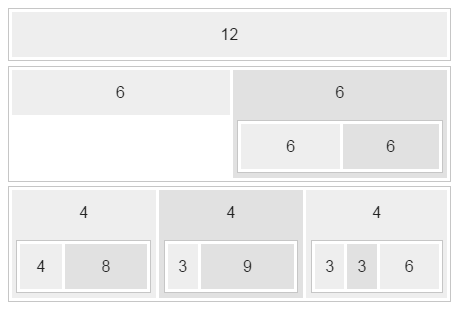
\includegraphics[scale=1]{Gambar/grid.png}
\caption[Gambar Contoh Grid]{Contoh Grid}
\label{fig:grid}
\end{figure}

\item Tombol\\
Mengklik tombol dengan material yang bagus merupakan hal yang mengagumkan. Mengklik tombol juga menghubungkan pengguna dengan berbagai aksi. Ada beberapa gaya tombol yamg ringan untuk ukuran, presentasi, dan warna untuk menyesuaikan tombol Anda sendiri semudah menambahkan kelas. Untuk contoh macam-macam tombol dapat dilihat pada Gambar \ref{fig:button}.

\begin{figure}[H]
\centering
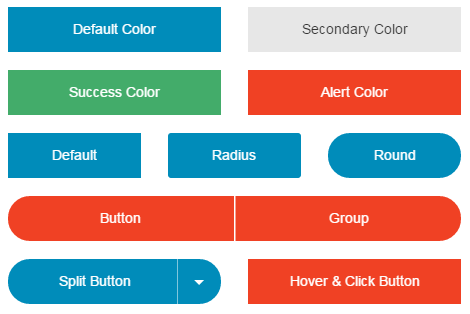
\includegraphics[scale=1]{Gambar/button.png}
\caption[Gambar Contoh Tombol]{Contoh Tombol}
\label{fig:button}
\end{figure}

\item Navigasi\\
Orang yang mengakses harus bisa berkeliling melihat menu-menu yang ada. Gaya navigasi pada Foundation meliputi : bar bagian atas yang kuat dengan menu dropdown; tombol; bar pencari; ikon bar yang keren; implementasi kanvas yang lepas dari keluhan; dan sekelompok navigasi lainnya. Untuk contoh macam-macam navigasi dapat dilihat pada Gambar \ref{fig:navi}.

\begin{figure}[H]
\centering
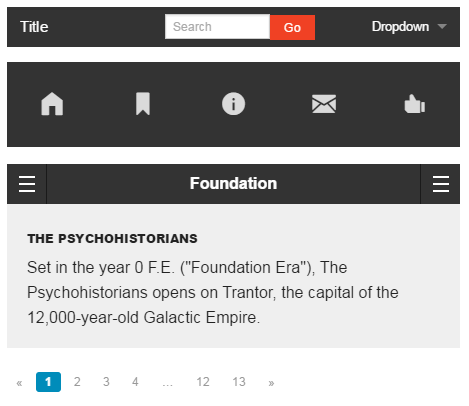
\includegraphics[scale=1]{Gambar/navigation.png}
\caption[Gambar Contoh Navigasi]{Contoh Navigasi}
\label{fig:navi}
\end{figure}

\item Plugins\\
Sudah meliputi banyak plugin javascript yang ditulis untuk modal dasar pop-up; menambat formulir validasi yang diperlukan; membuat tab konten; tanda peringatan; dan masih banyak lagi. Untuk contoh macam-macam plugin dapat dilihat pada Gambar \ref{fig:plugin}.

\begin{figure}[H]
\centering
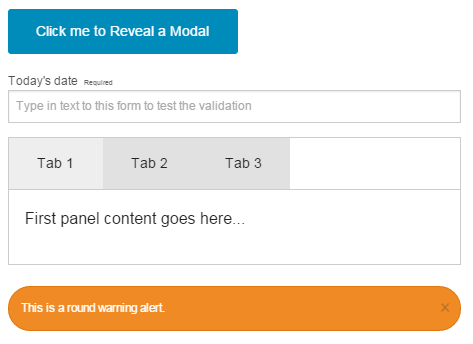
\includegraphics[scale=1]{Gambar/plugin.png}
\caption[Gambar Contoh Plugins]{Contoh Plugins}
\label{fig:plugin}
\end{figure}

\end{enumerate}